\chapter{Tutorial de utilização do supervisório didático} \label{Chap:Apendice1}

\section{Apresentação}

Esta seção contém um guia de utilização do supervisório didático, organizado em tópicos. Cada tópico descreve um passo-a-passo sobre como realizar as operações que o programa oferta.

\section {Primeira utilização}

O supervisório didático foi programado em linguagem Python e dividido em alguns arquivos, a fins de organização. Estes arquivos são agrupados e referenciados no script principal Supervisorio.py, sendo imprescidível que a organização dentro da pasta do programa não seja alterada. Caso seja, o script principal não conseguira encontrar os arquivos que contém as declarações de classes e será mostrado um erro no terminal.

Ao utilizar o programa, supõe-se que a máquina operante já possui Python instalado. O compilador pode ser baixado gratuitamente em \href{https://www.python.org/}{seu site oficial}. Os testes foram feitos com a versão 3.8.5 da linguagem, não sendo claros os efeitos que versões anteriores a esta causarão na operação.

Para intalação das bibliotecas utilizadas, roda-se o arquivo install\_packages.bat, presente na pasta utils. Talvez seja necessário permissão de administrador para executá-lo. Alternativamente, através do comando no código \ref{code_install_packages}, as bibliotecas listadas em requirements.txt será instaladas.

\begin{code}
	\begin{lstlisting}
	pip install -r requirements.txt
	\end{lstlisting}
	\label{code_install_packages}
\end{code}

\section{Iniciando o programa}

O script principal pode ser executado através de vários métodos, pois trata-se apenas de um script python. Para uma maneira rápida de fazê-lo, basta executar Supervisorio.bat. Ele não deve ser movido da pasta, mas pode ser criado um atalho para ele.

Quando o script é executado, a tela principal do supervisório aparecerá. Caso esteja presente um arquivo de salvamento automático autosave.dat no diretório raiz do programa, ele tentará restaurar as séries da sessão anterior. Caso apareçam erros no trecho que carrega estes dados, o usuário pode tentar deletar este arquivo.

\section{Importando séries estáticas no programa}

Existem diversos métodos de entrada de dados no supervisório. Primeiro, alguns parâmetros são configurados, de acordo com cada método, descritos nas subseções posteriores, e depois clica-se no botão "Puxar Dados".

\subsection{Função de Transferência}

A simulação de funções de tranferência no programa requer o numerador e denominador de cada função, multiplicadas entre sim, bem como o estado inicial da saída do sistema e o ganho do degrau aplicado. Para este método, o sistema reponde somente a uma entrada degrau. A entrada de dados por função de transferência se dá pelo objeto ilustrado na Figura \ref{img_transfer_func_config}.

\begin{figure}[!htb]
	\centering
	\caption{Objeto \emph{TransferFunctionConfig} (à esquerda)}
	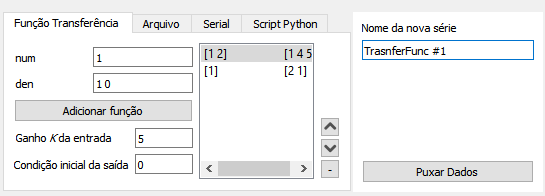
\includegraphics{transfer_func_config}
	\label{img_transfer_func_config}
\end{figure}

Com o campo num e den preenchidos com uma sequência de números separados por espaço, clica-se no botão "Adicionar Função" para incluí-la na lista à direita. Cada número é atribuído em ordem de posição a uma potência de s, sendo o número mais à direita atribuído a $s^0$. Como exemplo, um numerador "1 3" e denominador "2 0 1" representam a função de transferência $\frac{s + 3}{2s^2 + 1}$.

\textbf{OBS:} o numerador não pode ter grau maior que o denominador, por restrições da biblioteca empregada neste módulo.

A ordem das funções não impacta a resposta final, mas por questão de organização, foram incluídos botões à direita da tabela que mudam a posição de cada função na lista. O botão "-" remove a função selecionada, se houver, da mesma.

Terminada a entrada de funções de transferência, configuram-se o estado inicial e o ganho do degrau. Após isto, clica-se no botão "Puxar Dados"

\subsection{Entrada por arquivo}

O programa aceita 4 formatos de arquivos para inserção de séries, que são .csv, .tsv, .xls e .xslx. Todos estes formatos armazenam dados em tabela, logo compartilham seus parâmetros de importação:

\begin{itemize}
	\item \textbf{Cabeçalho:} Caso a opção "Considerar cabeçalho" seja marcada, o programa transformará a primeira linha de dados lida como a lista de nomes de cada série.
	\item \textbf{Eixo de tempo:} Com a opção "1ª coluna como eixo de tempo", o programa considerará a coluna mais a esquerda como eixo de tempo, compartilhado pelas outras séries contidas no arquivo. Caso a opção marcada seja "Gerar eixo de tempo autom.", o programa criaré este eixo pela quantidade de linhas lidas, começando em 1, e em incrementos unitários a cada leitura.
\end{itemize}

Na parte superior do objeto \emph{FileConfig}, são listados cada um dos formatos compatíveis com o programa. O formato selecionado configura o filtro de extensão do explorador de arquivos que aparece quando o botão "..." é clicado. Ao selecionar um arquivo por este explorador, o programa preencherá automaticamente os campos "Diretório" e "Arquivo".

\subsection{Serial}

A importação por porta serial é configurada pelos seguintes parâmetros:

\begin{itemize}
	\item \textbf{\emph{baud rate}}: velocidade de recebimento e transmissão dos dados na porta;
	\item \textbf{Porta}: nome da porta;
	\item \textbf{\emph{timeout}}: tempo máximo de resposta do dispositivo conectado, quando a comunicação for iniciada.
	\item \textbf{N\# colunas} quantas séries de dados recebidas devem ser esperadas pelo programa, incluindo a série de tempo. Após cada leitura da porta serial, se a quantidade de valores lidos diferir deste número, a leitura será desconsiderada.
\end{itemize}

Abaixo de algumas configurações existe uma lista com os valores mais populares de parâmetros. Ao clicar nos itens da lista, a caixa de texto será atualizada. O botão "Testar" abre e fecha uma conexão na porta informada, a fim de verificar se não houve problemas.

Para este caso, ao iniciar a importação, a janela de monitoramento irá aparecer, como descrito na seção \ref{monitoramento_tempo_real}.

\subsection{Script Python}

Esta alternativa busca oferecer aos usuários maneiras próprias de criação de dados. Na caixa de texto pode ser digitado um script python que retorne, nesta ordem, uma lista de séries, um eixo de tempo e uma lista de nomes. O programa criará um objeto \emph{SeriesObject} a partir do retorno deste script. Ainda é possível clicar duplamente na caixa de texto, momento no qual uma caixa maior aparece, garantindo maior visibilidade. Nela há também alguns exemplo de códigos, que podem ser modificados livremente pelo usuário.

A puxar dados de um script python, o programa escreve o texto em um arquivo denominado script.py, em seu diretório raiz, cuidando de toda a sixtaxe adicional. Em seguida, envia um comando ao sistema operacional para executar o script final, que armazena o resultado em um objeto serializado. Por fim, este objeto é decodificado e, caso não hajam erros, uma nova série é criada.

\section{Monitoramento em tempo real}\label{monitoramento_tempo_real}

Ao clicar em "Puxar Dados" por porta serial, o programa tenta estabelecer uma conexão com os parâmetros informados, na porta definida. O nome da porta pode variar com o sistema operacional.

Após a conexão ser estabelecida, o programa limpará qualquer informação escrita no buffer da porta e, em intervalos de 2 segundos nela escreverá "go", até que alguma informação de retorno seja recebida. Isso se repetirá até 100 vezes. Este procedimento por ser alterado na função \emph{setup\_connection()} do objeto SCADADialog, presente no script realtime\_objects.py na pasta objects.

Após esta rotina de sincronização, a função personalizada setup\_control() é chamada. Caso o usuário deseje enviar algum valor para o controlador (setpoints, parâmetros do sistema, entre  outros), deve fazê-lo por aqui. O programa abre também a janela de monitoramento \emph{SCADADialog}, com um gráfico que plota cada série de dados recebida em tempo real.

Finalmente, iniciam-se as rotinas de leitura da porta e atualização do gráfico, respectivamente a cada 0,2 e 1 segundo. Como mencionado, a rotina de leitura lê toda uma linha de dados da porta, divide-a pelas tabulações contidas, e atribui cada trecho a uma série de dados interna, sendo a primeira sempre o eixo de tempo. Este formato deve ser seguido pelo emissor, ou controlador, acoplado, pois caso não coincida com a quantidade de séries esperada passado como parâmetro, toda a linha será ignorada.

Contida na rotina de leitura está a função loop\_control(). Idealmente, ela tem como objetivo mandar valores para o controlador em tempo de execução.

Durante o monitoramento, o usuário pode interromper a execução ao clicar em "Parar" ou "Cancelar". O segundo fecha a janela de monitoramento e descarta a série armazenada até então. O primeiro somente interrompe u fluxo de dados, e possibilita que o usuário salve as séries lidas, clicando em "Criar Série".

\section{Salvando e editando séries de dados}

Qualquer que tenha sido o método de importação, o usuário terá uma visualização dos dados importados sempre antes de efetivamente salvá-los no programa. Isto é ilustrado na Figura \ref{img_edit_series_dialog}. 

Nesta caixa diálogo, o usuário pode editar o título do conjunto e cabeçalho de cada série sendo importada. Para editar o cabeçalho, clica-se no nome da série contido na tabela à esquerda e altera-se a caixa de texto imediatamente acima dela. Cada alteração deve ser confirmada com Enter.

Após realizadas as edições, o usuário pode clicar em "Criar Série", e ela aparecerá na lista de séries à direita da aplicação pricipal.

Para editar uma série já criada, clica-se no respectivo botão "Editar", na lista de série, e esta mesma janela aparecerá. Para este caso, o botão "Criar Série" será substituído por "Salvar Alterações".

\section{Plotando séries}

A plotagem de séries na área principal se dá clicando em "Plotar", momento no qual o gráfico no canto inferior esquerdo da aplicação desenhará a série, sem perder outras já plotadas. A legenda também será atualizada.

\section{Editando e exportando gráficos}

Abaixo da área de plotagem, existe uma barra com algumas opções de configurações, como:

\begin{itemize}
	\item 
\includegraphics[height=1em]{zoom_icon} Permite aplicar zoom no gráfico
	\item 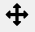
\includegraphics[height=1em]{move_icon} Permite mover o gráfico
	\item 
\includegraphics[height=1em]{home_icon} Retorna o gráfico à escala original
	\item 
\includegraphics[height=1em]{limits_icon} Configura o espaçamento do gráfico e sua moldura
	\item 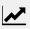
\includegraphics[height=1em]{axes_icon} Configura os eixos do gráfico, editando seu rótulo, limites e escala
	\item 
\includegraphics[height=1em]{save_icon} Salva o gráfico em formato de imagem
\end{itemize}

\section{Deletando séries}

Ao clicar em "Deletar", a série é apagada. Esta operação é irreversível.